\documentclass[]{article}
\usepackage{lmodern}
\usepackage{amssymb,amsmath}
\usepackage{ifxetex,ifluatex}
\usepackage{listings}
\usepackage{fixltx2e} % provides \textsubscript
\ifnum 0\ifxetex 1\fi\ifluatex 1\fi=0 % if pdftex
  \usepackage[T1]{fontenc}
  \usepackage[utf8]{inputenc}
\else % if luatex or xelatex
  \ifxetex
    \usepackage{mathspec}
  \else
    \usepackage{fontspec}
  \fi
  \defaultfontfeatures{Ligatures=TeX,Scale=MatchLowercase}
  \newcommand{\euro}{€}
\fi
% use upquote if available, for straight quotes in verbatim environments
\IfFileExists{upquote.sty}{\usepackage{upquote}}{}
% use microtype if available
\IfFileExists{microtype.sty}{%
\usepackage{microtype}
\UseMicrotypeSet[protrusion]{basicmath} % disable protrusion for tt fonts
}{}
\usepackage[margin=1in]{geometry}
\usepackage{hyperref}
\PassOptionsToPackage{usenames,dvipsnames}{color} % color is loaded by hyperref
\hypersetup{unicode=true,
            pdftitle={Untitled},
            pdfauthor={Andre Guimaraes Duarte},
            pdfborder={0 0 0},
            breaklinks=true}
\urlstyle{same}  % don't use monospace font for urls
\usepackage{color}
\usepackage{fancyvrb}
\newcommand{\VerbBar}{|}
\newcommand{\VERB}{\Verb[commandchars=\\\{\}]}
\DefineVerbatimEnvironment{Highlighting}{Verbatim}{commandchars=\\\{\}}
% Add ',fontsize=\small' for more characters per line
\usepackage{framed}
\definecolor{shadecolor}{RGB}{248,248,248}
\newenvironment{Shaded}{\begin{snugshade}}{\end{snugshade}}
\newcommand{\KeywordTok}[1]{\textcolor[rgb]{0.13,0.29,0.53}{\textbf{{#1}}}}
\newcommand{\DataTypeTok}[1]{\textcolor[rgb]{0.13,0.29,0.53}{{#1}}}
\newcommand{\DecValTok}[1]{\textcolor[rgb]{0.00,0.00,0.81}{{#1}}}
\newcommand{\BaseNTok}[1]{\textcolor[rgb]{0.00,0.00,0.81}{{#1}}}
\newcommand{\FloatTok}[1]{\textcolor[rgb]{0.00,0.00,0.81}{{#1}}}
\newcommand{\ConstantTok}[1]{\textcolor[rgb]{0.00,0.00,0.00}{{#1}}}
\newcommand{\CharTok}[1]{\textcolor[rgb]{0.31,0.60,0.02}{{#1}}}
\newcommand{\SpecialCharTok}[1]{\textcolor[rgb]{0.00,0.00,0.00}{{#1}}}
\newcommand{\StringTok}[1]{\textcolor[rgb]{0.31,0.60,0.02}{{#1}}}
\newcommand{\VerbatimStringTok}[1]{\textcolor[rgb]{0.31,0.60,0.02}{{#1}}}
\newcommand{\SpecialStringTok}[1]{\textcolor[rgb]{0.31,0.60,0.02}{{#1}}}
\newcommand{\ImportTok}[1]{{#1}}
\newcommand{\CommentTok}[1]{\textcolor[rgb]{0.56,0.35,0.01}{\textit{{#1}}}}
\newcommand{\DocumentationTok}[1]{\textcolor[rgb]{0.56,0.35,0.01}{\textbf{\textit{{#1}}}}}
\newcommand{\AnnotationTok}[1]{\textcolor[rgb]{0.56,0.35,0.01}{\textbf{\textit{{#1}}}}}
\newcommand{\CommentVarTok}[1]{\textcolor[rgb]{0.56,0.35,0.01}{\textbf{\textit{{#1}}}}}
\newcommand{\OtherTok}[1]{\textcolor[rgb]{0.56,0.35,0.01}{{#1}}}
\newcommand{\FunctionTok}[1]{\textcolor[rgb]{0.00,0.00,0.00}{{#1}}}
\newcommand{\VariableTok}[1]{\textcolor[rgb]{0.00,0.00,0.00}{{#1}}}
\newcommand{\ControlFlowTok}[1]{\textcolor[rgb]{0.13,0.29,0.53}{\textbf{{#1}}}}
\newcommand{\OperatorTok}[1]{\textcolor[rgb]{0.81,0.36,0.00}{\textbf{{#1}}}}
\newcommand{\BuiltInTok}[1]{{#1}}
\newcommand{\ExtensionTok}[1]{{#1}}
\newcommand{\PreprocessorTok}[1]{\textcolor[rgb]{0.56,0.35,0.01}{\textit{{#1}}}}
\newcommand{\AttributeTok}[1]{\textcolor[rgb]{0.77,0.63,0.00}{{#1}}}
\newcommand{\RegionMarkerTok}[1]{{#1}}
\newcommand{\InformationTok}[1]{\textcolor[rgb]{0.56,0.35,0.01}{\textbf{\textit{{#1}}}}}
\newcommand{\WarningTok}[1]{\textcolor[rgb]{0.56,0.35,0.01}{\textbf{\textit{{#1}}}}}
\newcommand{\AlertTok}[1]{\textcolor[rgb]{0.94,0.16,0.16}{{#1}}}
\newcommand{\ErrorTok}[1]{\textcolor[rgb]{0.64,0.00,0.00}{\textbf{{#1}}}}
\newcommand{\NormalTok}[1]{{#1}}
\usepackage{graphicx,grffile}
\makeatletter
\def\maxwidth{\ifdim\Gin@nat@width>\linewidth\linewidth\else\Gin@nat@width\fi}
\def\maxheight{\ifdim\Gin@nat@height>\textheight\textheight\else\Gin@nat@height\fi}
\makeatother
% Scale images if necessary, so that they will not overflow the page
% margins by default, and it is still possible to overwrite the defaults
% using explicit options in \includegraphics[width, height, ...]{}
\setkeys{Gin}{width=\maxwidth,height=\maxheight,keepaspectratio}
\setlength{\parindent}{0pt}
\setlength{\parskip}{6pt plus 2pt minus 1pt}
\setlength{\emergencystretch}{3em}  % prevent overfull lines
\providecommand{\tightlist}{%
  \setlength{\itemsep}{0pt}\setlength{\parskip}{0pt}}
\setcounter{secnumdepth}{0}

%%% Use protect on footnotes to avoid problems with footnotes in titles
\let\rmarkdownfootnote\footnote%
\def\footnote{\protect\rmarkdownfootnote}

%%% Change title format to be more compact
\usepackage{titling}

% Create subtitle command for use in maketitle
\newcommand{\subtitle}[1]{
  \posttitle{
    \begin{center}\large#1\end{center}
    }
}

\setlength{\droptitle}{-2em}
  \title{MSAN 502 - Homework 3}
  \pretitle{\vspace{\droptitle}\centering\huge}
  \posttitle{\par}
  \author{Andre Guimaraes Duarte}
  \preauthor{\centering\large\emph}
  \postauthor{\par}
  \predate{\centering\large\emph}
  \postdate{\par}
  \date{August 3rd, 2016}



% Redefines (sub)paragraphs to behave more like sections
\ifx\paragraph\undefined\else
\let\oldparagraph\paragraph
\renewcommand{\paragraph}[1]{\oldparagraph{#1}\mbox{}}
\fi
\ifx\subparagraph\undefined\else
\let\oldsubparagraph\subparagraph
\renewcommand{\subparagraph}[1]{\oldsubparagraph{#1}\mbox{}}
\fi

\begin{document}
\maketitle

\section*{Python problem}
In this problem, we will use \texttt{pandas} and \texttt{numpy} to find the best fit line in the sense of least squares to a set of data consisting of paired observations in the form $(x; y)$. The code for my implementation can be found in files \texttt{TVlife.py}, \texttt{population.py}, and \texttt{nba.py}. In addition, I found a data set online concerning XXX that I analyzed using the same system as these files. Here, I will explain how I proceeded, and show the results and graphs.

\subsection*{population.txt}
This file contains information concerning the national population ($y$) as a function of the year ($x$). Plotting $y$ against $x$, we get the graph seen in figure \ref{pop_plain}. We can see that a linear regression seems to be a likely candidate for regression.

\begin{figure}[h]
\centering
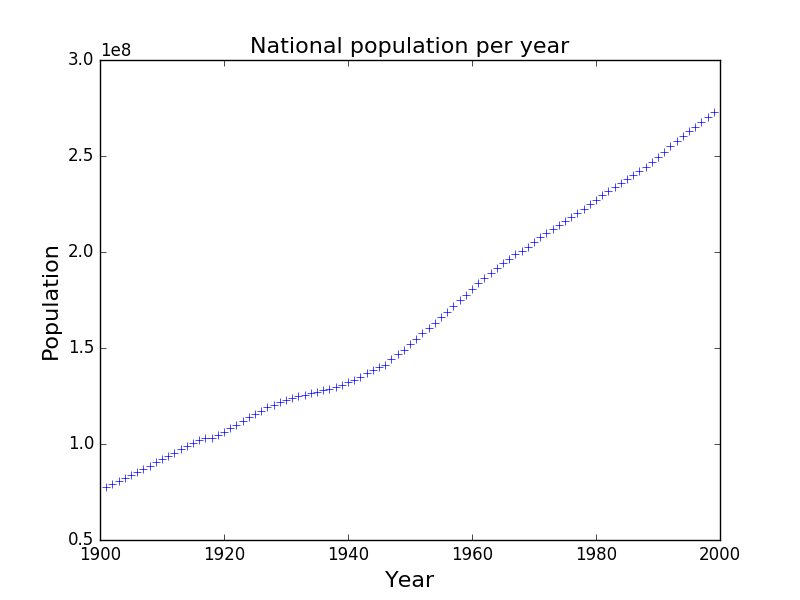
\includegraphics{pop_plain.png}
\caption{National US population from 1900 to 2000}
\label{pop_plain}
\end{figure}

With \texttt{numpy}, we can easily obtain $\widehat{\textbf{x}}$ that minimizes the error. We just need to compute:

$\widehat{\textbf{x}} = (A^TA)^{-1}A^T\textbf{b}$.

We get $\widehat{\textbf{x}} = \left[\begin{smallmatrix}-3.741 \cdot 10^9\\2.003 \cdot 10^6\end{smallmatrix}\right]$.

If we draw this line on top of the data, we get the image in figure \ref{pop_reg}.

\begin{figure}[h]
\centering
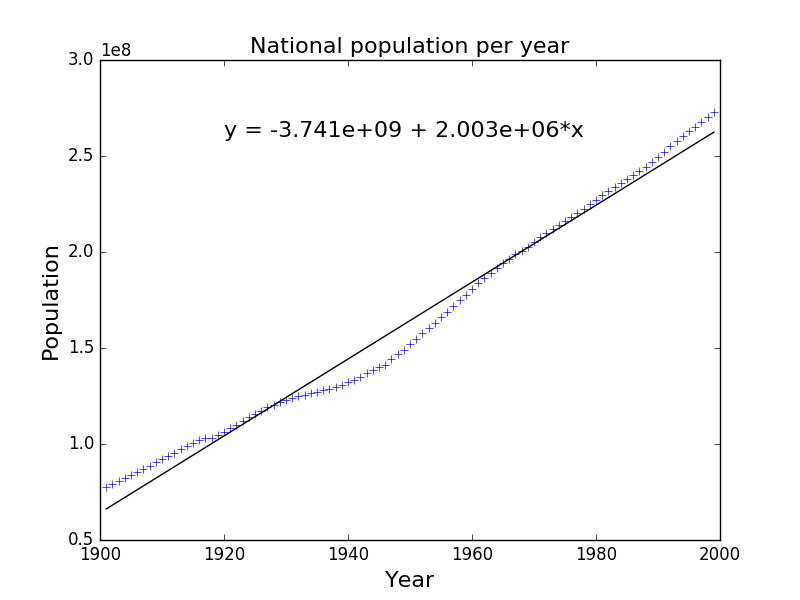
\includegraphics{pop_reg.png}
\caption{National US population from 1900 to 2000 and regression line}
\label{pop_reg}
\end{figure}

The fit that we computed seems to be what we would expect.

The error $\textbf{e}$ is found with the equation $\textbf{e} = \textbf{b} - A\widehat{\textbf{x}}$. In this case, we get $||\textbf{e}||^2 = 7.268 \cdot 10^7$.

\newpage
\subsection*{nba.txt}
This file contains information concerning team winning percentage in basketball games ($y$) as a function of PM (the average point difference over all that team's games) ($x$). Plotting $y$ against $x$, we get the graph seen in figure \ref{nba_plain}. We can see that a linear regression seems to be a likely candidate for regression.

\begin{figure}[h]
\centering
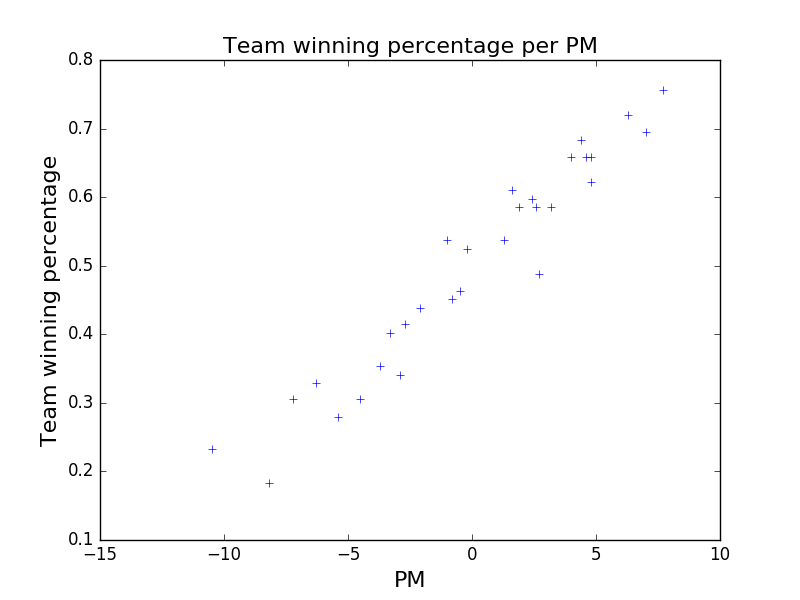
\includegraphics{nba_plain.png}
\caption{Team winning percentage as a function of PM}
\label{nba_plain}
\end{figure}

With \texttt{numpy}, we can easily obtain $\widehat{\textbf{x}}$ that minimizes the error. We just need to compute:

$\widehat{\textbf{x}} = (A^TA)^{-1}A^T\textbf{b}$.

We get $\widehat{\textbf{x}} = \left[\begin{smallmatrix}0.500\\0.032\end{smallmatrix}\right]$.

If we draw this line on top of the data, we get the image in figure \ref{nba_reg}.

\begin{figure}[h]
\centering
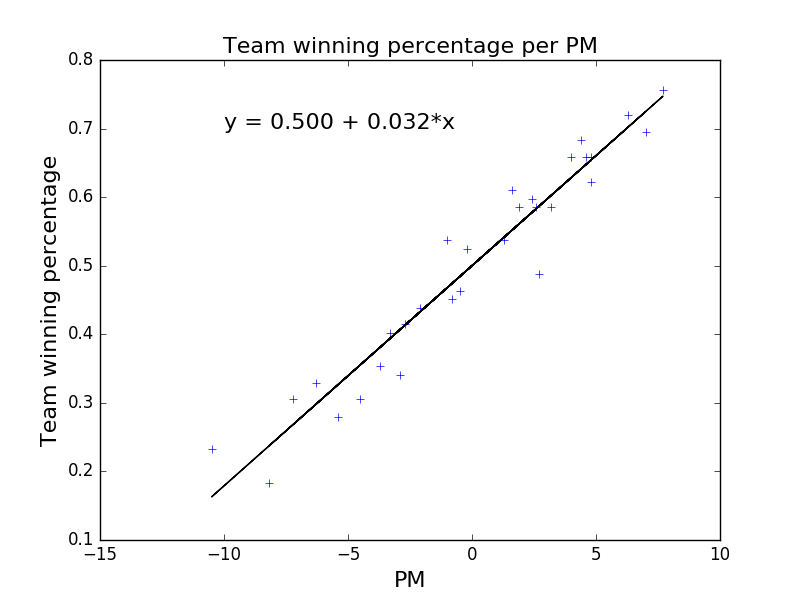
\includegraphics{nba_reg.png}
\caption{Team winning percentage as a function of PM and regression line}
\label{nba_reg}
\end{figure}

The fit that we computed seems to be what we would expect.

The error $\textbf{e}$ is found with the equation $\textbf{e} = \textbf{b} - A\widehat{\textbf{x}}$. In this case, we get $||\textbf{e}||^2 = 0.215$.

\newpage
\subsection*{TVlife.txt}
This file contains information concerning life expectancy ($y$) as a function of televisions per thousand people ($x$). Plotting $y$ against $x$, we get the graph seen in figure \ref{TV_plain}. In this case, linear regression does not seem like the best candidate for regression. Maybe a polynomial regression would work better in this case. But we will proceed with linear regression for this problem.

\begin{figure}[h]
\centering
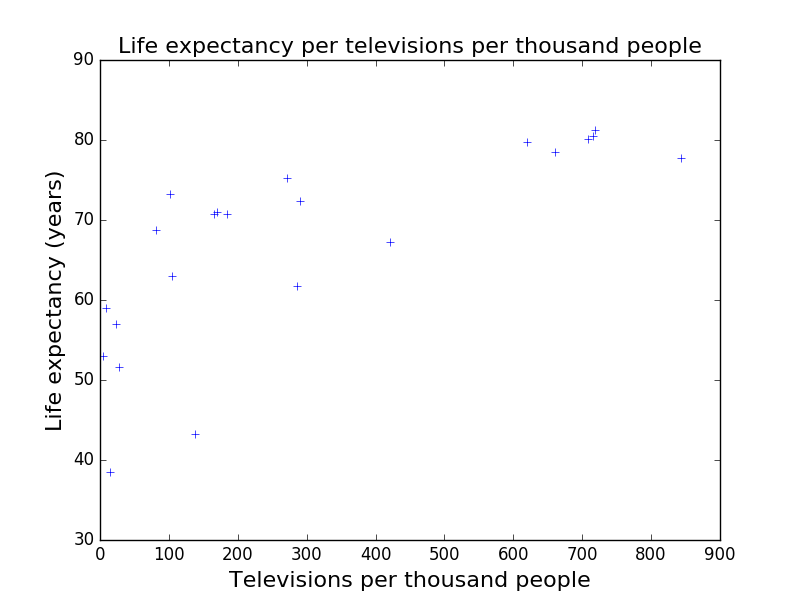
\includegraphics{TV_plain.png}
\caption{Life expectancy per televisions per thousand people}
\label{TV_plain}
\end{figure}

With \texttt{numpy}, we can easily obtain $\widehat{\textbf{x}}$ that minimizes the error. We just need to compute:

$\widehat{\textbf{x}} = (A^TA)^{-1}A^T\textbf{b}$.

We get $\widehat{\textbf{x}} = \left[\begin{smallmatrix}57.337\\0.032\end{smallmatrix}\right]$.

If we draw this line on top of the data, we get the image in figure \ref{TV_reg}.

\begin{figure}[h]
\centering
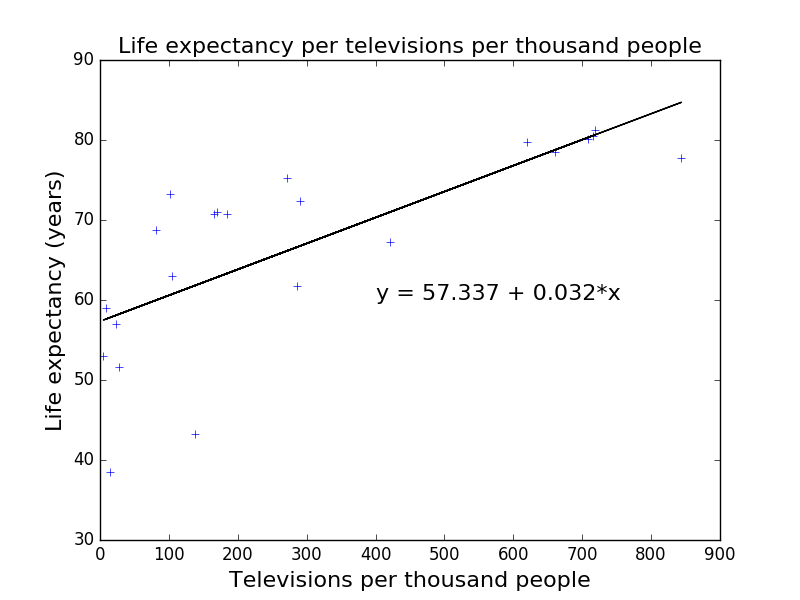
\includegraphics{TV_reg.png}
\caption{Life expectancy per televisions per thousand people and regression line}
\label{TV_reg}
\end{figure}

The linear fit seems adequate, but a polynomial regression would produce a better result in this particular case.

The error $\textbf{e}$ is found with the equation $\textbf{e} = \textbf{b} - A\widehat{\textbf{x}}$. In this case, we get $||\textbf{e}||^2 = 37.655$.

\newpage
\subsection*{30oysters.txt}
I got this file from the \textit{Journal of Statistics Education}, via the website \url{http://www.amstat.org/publications/jse/jse_data_archive.htm}. The file consists of 30 observations of 5 variables concerning oysters that was collected in 2001. The direct link to the file is: \url{http://www.amstat.org/publications/jse/datasets/30oysters.dat.txt}.

This file contains information concerning 30 oysters' volume in cc ($y$) as a function of their weight in grams ($x$). Plotting $y$ against $x$, we get the graph seen in figure \ref{30oysters_plain}. We can see that a linear regression seems to be a likely candidate for regression. The data seems very linearly correlated.

\begin{figure}[h]
\centering
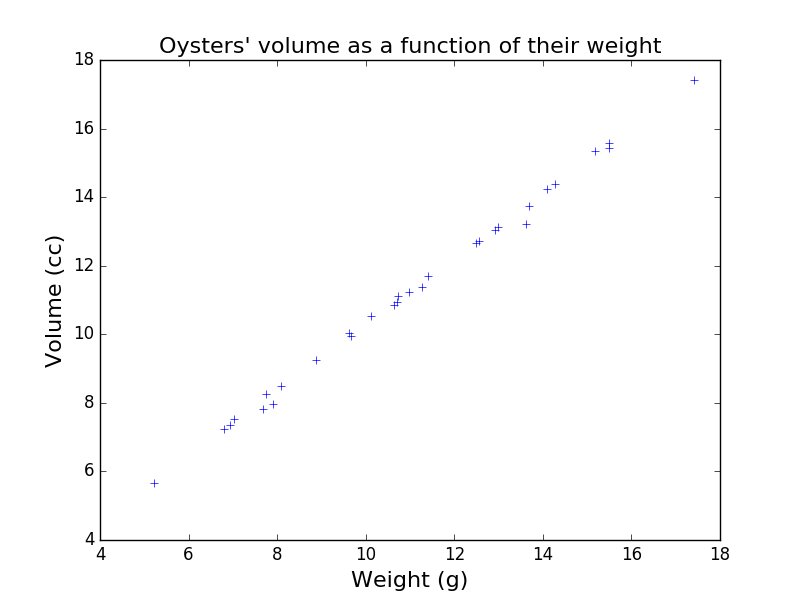
\includegraphics{30oysters_plain.png}
\caption{Oysters' volume as a function of their weight}
\label{30oysters_plain}
\end{figure}

With \texttt{numpy}, we can easily obtain $\widehat{\textbf{x}}$ that minimizes the error. We just need to compute:

$\widehat{\textbf{x}} = (A^TA)^{-1}A^T\textbf{b}$.

We get $\widehat{\textbf{x}} = \left[\begin{smallmatrix}0.714\\0.955\end{smallmatrix}\right]$.

If we draw this line on top of the data, we get the image in figure \ref{30oysters_reg}.

\begin{figure}[h]
\centering
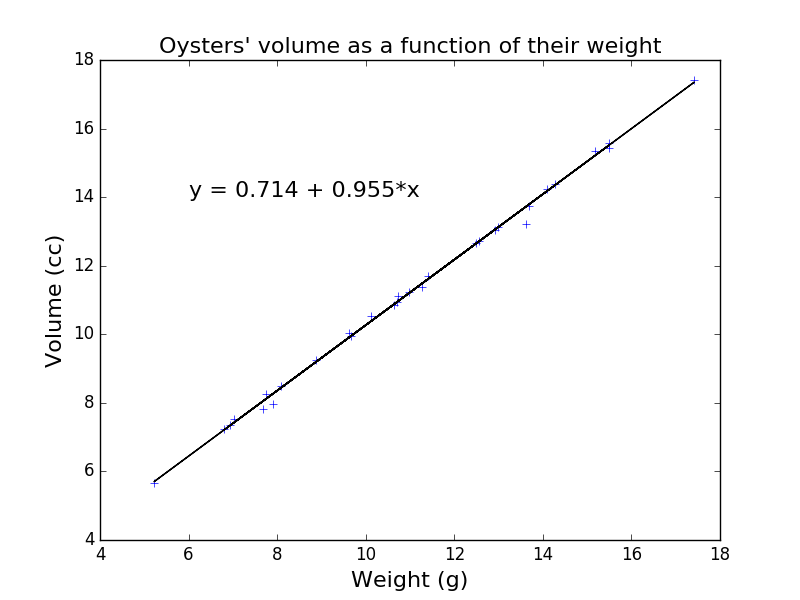
\includegraphics{30oysters_reg.png}
\caption{Oyster's volume as a function of their weight and regression line}
\label{30oysters_reg}
\end{figure}

The fit that we computed seems to be what we would expect.

The error $\textbf{e}$ is found with the equation $\textbf{e} = \textbf{b} - A\widehat{\textbf{x}}$. In this case, we get $||\textbf{e}||^2 = 0.758$.

\end{document}
